% !Mode:: "TeX:UTF-8"

\chapter{基于深度学习的声学建模}\label{intro_dl}


深度学习在语音识别中的引入,替代了经典HMM-GMM系统中采用GMM对状态概率密度进行建模的方法,
使用深度神经网络对状态的概率分布进行建模,称之为基于HMM-DL(HMM-Deep Learning)的语音识别系统。

本章介绍深度学习的基本原理和在语音识别中的基本应用。以下介绍几种常见的神经网络结构全接连的神经网络DNN、
卷积神经网络CNN、循环神经网络RNN等深度学习网络的基本结构;
研究这些深度学习网络在语音识别这个特定任务中的使用方式,改进和组合使用(CLDNN)等;
最后本章给出这几种深度学习方法的相关实验。

\section{HMM-DL系统}\label{section:hmmdl}

在经典HMM-GMM的语音识别系统中,为每个状态建立一个GMM模型来描述其概率分布,
在识别时,通过各自状态的GMM可以直接计算$t$时刻的观测$o_t$在状态$s_i$上的概率
$p(o_t|s_i)$,$p(o_t|s_i)$HMM系统识别时必须的依赖。

深度学习引入语音识别后,使用深度神经网络来替代GMM对每个状态进行建模,
在深度神经网络中,这是一个典型的分类任务,即当新的一帧语音到来时,
通过深度神经网络计算其在每个状态上的概率。
与GMM系统为每个状态建立独立的GMM模型不同,深度神经网络本身为紧凑模型,即所有状态共享一个模型。
通过深度神经网络直接计算出的是$p(s_i|o_t)$,而非$p(o_t|s_i)$,
这是基于GMM和神经网络对声学模型进行建模的一个本质上的不同。

通过贝叶斯公式有:
\begin{equation}
p(o_t|s_i) = \frac{p(s_i|o_t)p(o_t)}{p(s_i)}
\end{equation}
在识别的解码过程中,为防止概率连乘导致下溢,概率计算一般转到$log$域,取$log$有:
\begin{equation} \label{equation:hmmdnn}
\log{p(o_t|s_i)} = \mathop {\log{p(s_i|o_t)} + \log{p(o_t)} - \log{p(s_i)}} \\
\;\;\;\;\;\;\;\;\; = \mathop {\log{p(s_i|o_t)} - \log{p(s_i)}}
\end{equation}
其中$p(o_t)$为$o_t$发生的概率,对所有的状态相同,因此可以忽略。
$p(s_i)$为状态$s_i$出现的概率,称之为状态先验,一般可以通过对训练数据集作状态统计得到。
通过公式\ref{equation:hmmdnn},便可以计算得到$p(o_t|s_i)$,这便是基于HMM-DL系统进行语音
识别的基本原理。



\section{全连接神经网络DNN}

深度神经网络DNN\ucite{bengio2012practical}(Deep Neural Network)是有多个(一般均大于2层)隐层的传统的多层感知机MLP(MultiLayer Perceptron)。
一个典型的神经网络由输入层;中间多个隐层和输出层组成。
如图\ref{fig:dnn}所示DNN,含有3个隐层,每个隐层有5个节点。
在一个$L+1$层的DNN中,我们定义输入层为第$0$层,输出层为第$L$层。

\begin{figure}
\centering
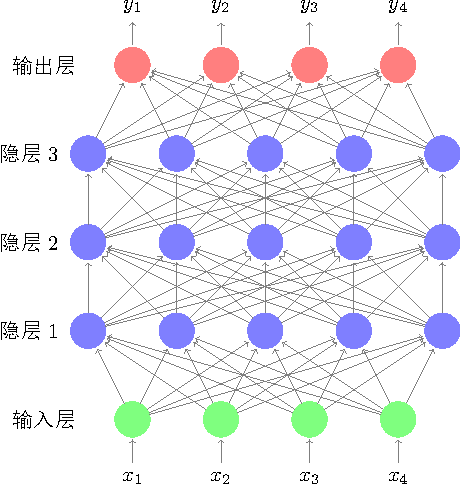
\includegraphics[width=0.5\textwidth]{figures/chapter3/dnn-crop}
\caption{DNN示例(该DNN由输入层、3个隐层和输出层组成)}
\label{fig:dnn}
\end{figure}

对于任意隐层$l$的任意节点$j$,有:
\[\begin{array}{l}
a_j^l = \sum\limits_{i = 1}^N {w_{ji}^l {x_i}^{l-1}+ b_j^l} \\
z_j^l = h(a_j^l)
\end{array}\]

其中,$i = 1,...,N$表示$l-1$层的节点数目,$a_j^l$表示第$l$层第$j$个节点的激励,
$a_j^l$经过激活函数$h(.)$作用得到$z_j^l$。
通常$h(.)$为非线性的、可导函数,
通过非线性函数增强神经网络的非线性映射能力,可导性则可以使神经网络通过梯度的方法行优化。

\subsection{激活函数}

在深度神经网络的实际应用中,最常用的激活函数是$sigmoid$函数:
\begin{equation}
s(z) = \frac{1}{{1 + {e^{ - z}}}}
\end{equation}
或者$tanh$函数:
\begin{equation}
\tanh (z) = \frac{{{e^z} - {e^{ - z}}}}{{{e^z} + {e^{ - z}}}}
\end{equation}
$sigmoid$函数将输入通过非线性函数映射到空间$(0,1)$;$tanh$函数的值域空间为$(-1,1)$,
其映射空间具有对称性。$ReLU$\ucite{glorot2011deep}是近年深度学习技术流行之后,又一个非常有效的激活函数:
\begin{equation} \label{equation:relu}
{\mathop{\rm Re}\nolimits} LU(z) = \max (0,z)
\end{equation}
$ReLU$激活函数预测具有稀疏性,这中预测特性提高了网络的泛化能力;另一方面,
如式\ref{equation:relu},$ReLU$的梯度形式简单,非0即1,有效的缓解了深度神经网络
训练中的梯度弥散问题;而且$ReLU$激活函数的计算更加简单,速度更快。
三种激活函数如图\ref{fig:activation}所示。

\begin{figure}
\centering
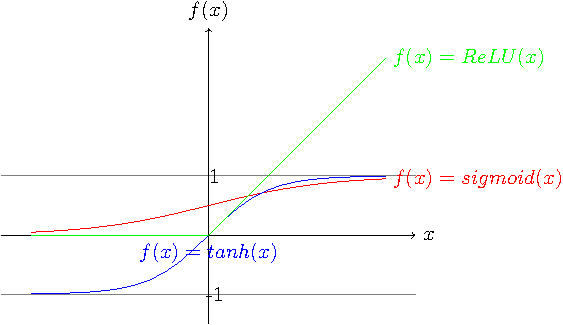
\includegraphics[width=0.6\textwidth]{figures/chapter3/activation-crop}
\caption{激活函数$sigmoid$,$tanh$,$ReLU$对比}
\label{fig:activation}
\end{figure}

激活函数的选择和深度神经网络密切相关,因此设计更好的激活函数也成为当下深度学习研究的热点之一,
最近的实验\ucite{zhang2014improving, zhang2015parameterised}表明,经过精心设计的激活函数能够
在一定程度上提高深度神经网络的性能。

\subsection{DNN训练}

DNN的训练即在损失函数确定后,使用误差方向传播BP(Back Propagation)算法计算参数梯度,
使用随机梯度下降SGD(Stochastic Gradient Descent)对模型中的参数进行更新。

一般来说,对于回归任务,使用最小均方误差MSE(Mean Suqare Error)损失函数:
\begin{equation}
E({\rm{w}}) = \frac{1}{2}\sum\limits_{n = 1}^N {\{ {y_n}}  - {t_n}{\} ^2}
\end{equation}
其中$y_n$为网络输出,$t_n$为标注,$N$为样本总数。

对于分类任务,首先应用$softmax$函数:
\begin{equation}
{y_k} = \frac{{\exp ({a_k})}}{{\sum\limits_j {\exp ({a_{\rm{j}}})} }}
\end{equation}
计算在每个类别上的归一化后的概率,然后使用交叉熵CE(Cross Entropy)准则计算损失:
\begin{equation}
E(w) =  - \sum\limits_{n = 1}^N {\sum\limits_{k = 1}^K {{t_{kn}}\ln {y_k}} }
\end{equation}

根据\ref{section:hmmdl},基于深度神经网络的声学建模为典型的分类任务,
在输出层使用$softmax$函数做概率归一,使用交叉熵作为损失函数。

\section{卷积神经网络CNN}

\section{循环神经网络RNN}

\section{混合神经网络CLDNN}

\section{实验} 